\providecommand{\main}{..}
\documentclass[\main/master.tex]{subfiles}
\begin{document}
\chapter{thesis aims}\label{chp:example-2}
\section{Measurement Method}
The Cavendish experiment, is constructed using a torsional pendulum with a front mirror. The angle displaement is causing a mirror tilt. Optical measurement of angle displaement is made with a split detector. 
\par
Shot noise using a split detector in an interferometric technique is even on all frequencies. Shot limit when integrating over a long time.
\begin{equation}
\Delta\theta = \frac{1}{4\sqrt{2}\pi}\frac{\lambda}{L\sqrt{N}} \approx
4\cdot10^{-14} [\frac{rad}{Hz}]    \label{eqn:gravitation_tourqe}
\end{equation}
When the gravitational force is measured using a torsional pendulum, there are noise limitation to the measuremnt sensetivity. The limitation are higher than the shot noise limit, meaning that reducing the noise could achieve higher sensetivity. The noises on the pendulum are unknown magnetic noise, acoustic waves and random fluctuations due to thermal brownian motion.Friction is also limiting the pendulum response. 
\par
Pendulum is placed inside vacuum reducing brownian motion, acoustic waves and friction, vacuum chamber is reducing magnetic noise by faraday cage. At vacuum the brownian motion from envirement coupling is reduced, but still is the main noise source. The system quantum uncertainty at a specific temperature due to brownian motion (assuming noise is much higher than basic energy level). 
\begin{equation}
\frac{1}{2}\kappa (\delta\theta_{max})^2= \frac{1}{2}KT  \label{eqn:radiation force}
\end{equation}
\begin{equation}
\delta\theta_{max} = \sqrt{\frac{KT}{\kappa}}\propto{T}  \label{eqn:radiation force}
\end{equation}

The noise reductance enables to damp and cool the pendulum temperture. Damping is made using a PID feedback loop. The feedback damping can dynamically damp the noises, without pre-knowledge of the existing noises. PID would reduce all noises, and reduce the temperature. Having an effective lower temperature would enable measuring smaller angles enlarging the SNR and the measuremnt sensetivity.
\par
When damped pendulum ossiclations become smaller, PID error is getting samller and damping response becomes small. 
\begin{equation}
e(t) = \delta\theta(t)   \label{eqn:pid_error}
\end{equation}
\begin{equation}
u(t) = K_Pe(t)+K_I\int_{0}^{t}e(t)+K_D\frac{de(t)}{dt}   \label{eqn:PID_eq}
\end{equation}

Introducing a new mass adds a constant new tourqe to the system, which the PID is compensating with a propotional gain $K_P$. The PID response becomes mainly an inverse tourqe. 
\begin{equation}
e(t) = \delta\theta(t) + \theta_g(t)    \label{eqn:PID_measurement}
\end{equation}
\begin{equation}
u(t) = u[ \delta\theta(t)] + K_P\theta_{gravity} \label{eqn:PID_measurement_eq}
\end{equation}
\begin{equation}
U = \int u(t)dt  \approx K_P\theta_g \label{eqn:PID_measurement_eq}
\end{equation}
\begin{equation}
\tau(r) = L\frac{GmM}{r^2} =  \kappa\theta_g = \kappa\frac{U}{K_P}      \label{eqn:pid_gravitation_tourqe}
\end{equation}
\begin{equation}
\kappa =\frac{8\pi^2ml^2}{T^2}    \label{eqn:empirical_tourqe}
\end{equation}
The measurement of that response is fast and accurate. The measurement sytem is measuring with fast response (short integration time) and high accuracy low frequency garvity fields. 

\section{PID}
\subsection{Damped Oscillator}
PID controller can continuously calculates error value of an oscillator, to damp it to zero. If the defined set point is set to zero, the error is the measured process variable. The PID acts as friction, gradually working when the ossicilations are at the maximum speed to slow them down, and remove the tourqe energy.
\begin{equation}
e(t) = \theta(t) = \theta   \label{eqn:error}
\end{equation}
\begin{equation}
\tau_{PID} = -\gamma\cdot\dot{\theta}   \label{eqn:friction_tourqe}
\end{equation}
The sytem is a damped oscillator, with an external force correction, which inserts tourqe to the oscillator.
\begin{equation}
\kappa\cdot\theta - \gamma\cdot\dot{\theta}  + I\cdot\ddot{\theta} = 0   \label{eqn:damped__pid_motion_equation}
\end{equation}
\begin{equation}
\gamma\dot{\theta}  = Fr   \label{eqn:damped__pid_motion_equation}
\end{equation}
\begin{equation}
\dot{\theta} = \omega_0\theta_{max}sin(\omega_0 t +\phi)    \label{eqn:undamped_motion_equation}
\end{equation}
\begin{equation}
\dot{\theta}_{max} = \omega_0\theta_{max} = \theta_{max}\cdot\frac{2\pi}{T}    \label{eqn:undamped_motion_equation}
\end{equation}
\begin{equation}
\gamma  = \frac{F_{max}r}{\dot{\theta}_{max}} =\frac{F_{max}rT}{\theta_{max}2\pi}    \label{eqn:damped_pid_motion_equation}
\end{equation}
\begin{equation}
\tau =  \frac{2I}{\gamma}  \label{eqn:damping_time}
\end{equation}
The PID damping $\gamma$ and damping time $\tau$ depends on the initial oscillations angle. If the angle is too large compare to the inserted force, the system is extremly underdamped and the PID affect is neglected. The damping time would be infinite and the system would keep on ossicilating.

\subsection{Control Stability}
Using PID control does not guarantee optimal control or stability. The control system is aiming to achieve critical damping of the process. Well tuned control would a reach the desired set point fast and accurate, and also apply over time the nesseary corrections to resist external forces trying to move variable from the set point.
\par
The controller response is its response to error. How much does the sytem overshoots a setpoint and the system oscillations. When controller gains are too high, instead of critical damping there is overdamping causing overshoot, due to the high gain the overshoot response overshoots to the other side, causing the system to be driven.
\subsection{Radiation Pressure Force}
The pendulum is cooled down using radiation pressure force. Fast modulated light source with high intensity cause a small controlled force. The diffrence between two light sources from both ends of pendulum adds a controled small damping tourqe. 
\begin{equation}
F = \frac{2\eta\Theta}{{c}} \label{eqn:radiation force}
\end{equation}
\begin{equation}
\tau\approx d\Delta F = \frac{2d}{{c}} (\eta_1\Theta_1 -\eta_2\Theta_2) \label{eqn:radiation tourqe}
\end{equation}
The radiation pressure tourqe assuming light fields direction perpendicular to surface, $\Theta$ is the light source radiant flux [watt], and $\eta$ is the coupling efficiency. The center of mass distance from rotation axis $d$ of both forces is even.
\par
The setup could produce very small tourqes; light sources of 1 watt maximum power and 8bit modulation steps could produce nano-$N\cdot m$ to pico-$N\cdot m$ tourqes. 

 
 
 
 





\section{accuracy}
\doublespacing
\hspace{5 mm} This another example chapter with a working reference as see in Chapter~\ref{chp:example-1}. There I also made an example of an equation, see Eqn.~\ref{eqn:energy-mass-equivalence-relation}. We also created an example image, see Fig.~\ref{fig:sine-wave}.
\begin{figure}[htbp]
	\centering
	\fbox{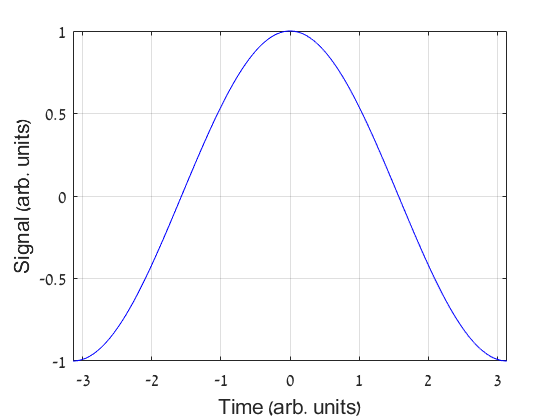
\includegraphics[scale=0.75]{\main/images/chapter_2_example/img_example_2.png}}
	\caption[Another Example Image]{Another Example Image. This image is also labeled internally so we can referenc it throughout the text.}
	\label{fig:cosine-wave}
\end{figure}
\end{document}